%This chapter will be about the dynamics of modelled NPS. Mostly the former part of the Nanoscale paper. I would like to include as much of the CNAP data as possible too
%I think that this chapter should be the 4th one and swap with the DFT
% 1. This will be the first bit of the nanoscale paper. introducing the structures used and why these in particular.
% 2. Next will be ALL off the alloying work I have. Motivating the choice of metals in the project and why these given alloys and configurations.
%   2.1 Let's just focus on the annealing and what this means for the energetics if the NPs and so on.
% 3. This will be all of the NEB calculations I have performed. what we can judge from them and what they mean.
% 4. This will be all about the effects of an environment on the AuPt nanoparticle - attempting to create a model which is able to emulate a water environment.

%Sec 5.1 Report here what type of simulation you have performed 
%--- the main idea
%--- the table with initial and final
%Sec 5.2 
%Report the reconstructions/reordering you observe

%Sec 5.3
%You might want to add here a comment on the diffusion properties. I have tried to understand your graph but I have no data %related to them.
%briefly... what we want is
%- to see a difference between the Au-seed morphology and that the barriers can be thermally activated. 
%But the mechanisms considered were not clear.

%Sec 5.4
%Add here the GDM calculations of the optical spectra  during the dynamics or at relevant snapshots/configurations
\noindent\enquote{\itshape When in doubt, go to the library. }\bigbreak

\hfill Ron Weasley - Harry Potter and the Chamber of Secrets

\vspace*{0.05\textheight}

In this chapter we shall present the, as of yet, unpublished work concerning vacuum state coalescence processes of AuPt nanoalloys. We evaluate various chemical orderings, initial morphologies, and relative abundances of the two species with respect to the structural stability and longevity of each sample. We shall present the results of canonical ensemble classical molecular dynamics, presented in Section \ref{sec:CMD}; and the classically computed optical extinction spectrum for each sample - drawing comparisons with experimental data presented in \cite{JorgeStructure}.

In brief, the aim of this chapter is to determine how composite AuPt nanoalloys may evolve subject to fixed temperature dynamics and what effect these dynamics may have on the photo-extinction spectrum drawing comparisons with experimental observations.

\section{Coalescence of Au and Pt nanoparticles}
%
Here we analyse the chemical stability of small Pt-nanoparticles decorating larger Au-nanoparticles, with a focus on Pt-loading between 2-50\%, over several hundreds of ns. We model the decoration as a soft deposition process, and we investigate several scenarios to elucidate the effect of the Au-core morphology, temperature, Pt-loading and different decoration patterns. 

%
We perform classical molecular dynamics simulations, using the open-source package LoDiS \cite{LoDiS}, at fixed temperature using an Andersen thermostat with a frequency of 10$^{11}$Hz. Inter-atomic potentials are modelled within the 2$^{nd}$ moment approximation of the tight binding (SMATB potentials, otherwise named RGL, or Gupta) \cite{RGL} with the parameters used tabulated in Table \ref{tab:RGL}.  These potentials have been used widely in the community \cite{LaiaMelt,AgPdAuPdAuPt}, therefore our results should be consistent and reproducible. 
We have elected to adopt a soft-landing approach as in Ref. \cite{Gazzarrini2021}, with  near-zero momentum interaction between the Au seed and the Pt decoration.

\begin{figure}
    \centering
    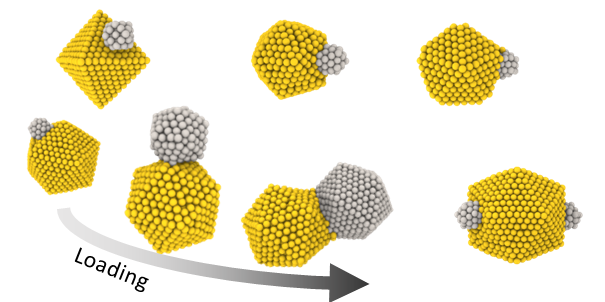
\includegraphics[width=\textwidth]{figures/MD/AuPt_beginning.png}
    \caption{Simplified scheme to depict the various considered cases. Top panel: "morphology effect" a Pt$_{55}$ is soft-landed onto Au-Oh$_{891}$ ; Au-Ih$_{923}$, Au-Dh$_{1103}$. Bottom: "loading effect" various size Pt-Ihs are soft landed onto 'magic'-size of Au-Ih, here Ih$_{561}$. Pt size varies between 55 and the size of Au. Bottom right: complex decorating pattern, as two Pt-Ih$_{55}$ soft-landed onto opposite facets of a Au-Ih$_{2057}$.}
    \label{fig:beginning}
\end{figure}

We consider three sets of simulations, as schematically depicted in Figure \ref{fig:beginning}, addressing the effects of: (i) the Au-core morphology; (ii) the Pt-loading; (iii) complex Pt-decoration - two identical Pt clusters decorating the same Au seed. In each iteration, we consider the effect of temperature, as adatom surface diffusion mechanisms and whole reconstruction are thermally activated processes. Nonetheless, we have generally elected to conduct our dynamics at higher temperatures than is common in laboratory environments \cite{Jorge2019,Jorge2021,JorgeStructure} so as to accelerate the rate at which mechanisms may either be activated or be conducted. This is a common practice and is more commonly known as Temperature Accelerated Dynamics (TAD) \cite{doi:10.1146/annurev-chembioeng-080615-033608}. 
%

We consider Au-core with a octahedral (Oh), decahedral (Dh) and icosahedral (Ih) morphology. We limit our analyses to geometrically closed shapes. However, we do not expect that limiting our analysis to closed shapes only will profoundly influence our conclusions. Figure  \ref{fig:Ptload_Struts} shows set of typical initial and final configurations: (i) Pt$_{55}$ on Au-Oh$_{891}$, Au-Ih$_{923}$, Au-Dh$_{1103}$ all at 600K, 450K, and 300K; (ii) Pt$^{Ih}_{n}$ on Au$^{Ih}_{N}$ at magic sizes $_{N,n}$ N = 55, 147, 309, 561, 923, 1415, and n = 13, 55, 147, 309, 561,923, 1415 at 600K; (iii) two Pt$_{55}$ on Au-Ih$_{2057}$ at 600K.
%%%%%%%%%%%%%%%%%%%%%%%%%%%%%%%%%%%%%%%%%%%%%%%%%%%%%%

We average our results over four independent simulations for every system and temperature considered so that we may collect statistics from independent realisations to ensure a greater reliability. For each of the subsequent figures, uncertainties are given as broader regions in the time-dependent curves or as error bars where a single point is being considered. These uncertainties are simply the standard error from considering several identically and independently realised iterations of the same process.

We compute local, semi-local, and global structural descriptors to monitor the evolution of the Pt-decorated Au-NPs and to determine when there are significant transitions in the atomic environments. An atomic environment is defined within a dynamically variable cutoff radius determined by the first minimum of the PDDF as defined in Chapter \ref{c:Sapphire}.

%
\begin{figure}
    \centering
    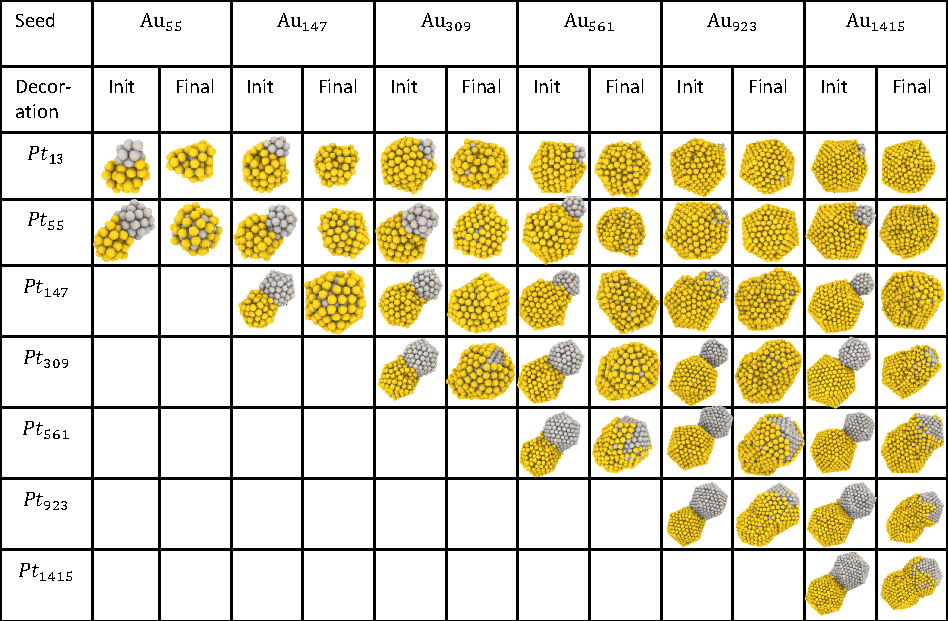
\includegraphics[width=\textwidth]{figures/MD/Coal/Ih_Struts.pdf}
    \caption{Exemplary snapshots of initial and final configurations of the Ih-Ih interaction of AuPt nanoalloys.}
    \label{fig:Ptload_Struts}
\end{figure}

We monitor, with respect to time, the chemical ordering, and attempt to identify possible reordering mechanism(s). To achieve this, we calculate the following descriptors:
\begin{itemize}
    \item $Pt_{Surf} / Pt_{Iso}$ - number of surface Pt atoms relative to the expected number for an isolated NP of the same morphology. Here, we adopt a simple definition to classify a surface atom based on its aGCN $\leq$ 9.
    \item $\langle Pt^{NN}_{n} \rangle$ - average coordination of Pt atoms in a cluster of size $n$ divided by the maximum coordination in the bulk (here a 12 as the reference is an FCC). A fast indicator for recognising when the Pt NP becomes encapsulated. For reference, a free Pt-Ih$_{55}$,  $\langle Pt^{NN}_{n} \rangle \sim 0.71$, against a value of 1 when fully encapsulated.
    \item $LAE^{Pt}_{Au = m}$ - local atomic environment of each Pt atom. It provides how many Pt atoms, with respect to the Pt initial amount, have $m$ Au as nearest neighbours, defined by the dynamically variable cutoff radius. Specifically, we report $m=0$, occurrence of Pt-atoms without any Au nearest neighbours, and $LAE^{Pt}_{Au \geq 10}$, identifying Pt atoms approaching encapsulation with respect to Au. With the former indicating the Pt NP remains phase separated with respect to the Au seed; while the latter becoming non-zero indicates that Pt atoms may be rearranging to form a partial-shell within the Au seed\cite{Hong2019}.
    \item $\Delta CoM$ - is the signed change in distance between the centre of mass (CoM) of the Pt decoration from the CoM of the full system, relative to the instant when the Pt decoration touches the Au seed.
    
\end{itemize}


\subsection{Au-morphology effect}

In our first investigation, we consider only three fixed thermostat temperatures to represent cold (300 K), mild (450 K), and warm (600 K) systems. Given that, in general, a system will attempt to evolve such that it enters a global minimum with respect to the potential energy one may assume that at infinite time at a fixed temperature, the structures will evolve to identical states. However, the objective here is not to determine the configuration of the global energy minimum, as there exist more efficient methods for determining such a state. For example, either a genetic algorithm \cite{YANG2018371,Fra_Ricardo_Review,Oakley2013-zl} or basin hopping \cite{Fra_Review,B204069G,doi:10.1021/jp207246m} are commonly used methods to achieve such results. Rather the aim is to determine within a finite time, how we may expect the system to evolve, much as it would if it were being measured under experimental conditions. Given this condition, we expect each considered nanoalloy at a given temperature to evolve towards a local energy minimum where it may spend long periods of time appearing stable. 

We begin by considering only a small subset of seed Au clusters: Au$_{1103}^{MDh}$, Au$_{923}^{Ih}$, and Au$_{891}^{Oh}$. Each of an approximately similar size and dimensionality, but exhibiting variation in their surface and core features, so as to be consistent. Each of these is decorated with one of two small Pt clusters Pt$_{55}^{Co}$ or Pt$_{55}^{Ih}$. As stated before, this is to emulate a simplified and miniaturised version of the structures described in \cite{Jorge2019}. Each structure is permitted to evolve dynamically subject to the Andersen thermostat set to either 300 K, 450 K, or 600 K for 500 ns to ensure that a sufficiently representative set of dynamics have been monitored. Prior to each realisation, a brief 1 ns thermalisation period occurs but has not been reported. 

\begin{figure}
     \centering
     \begin{subfigure}[b]{0.31\textwidth}
         \centering
         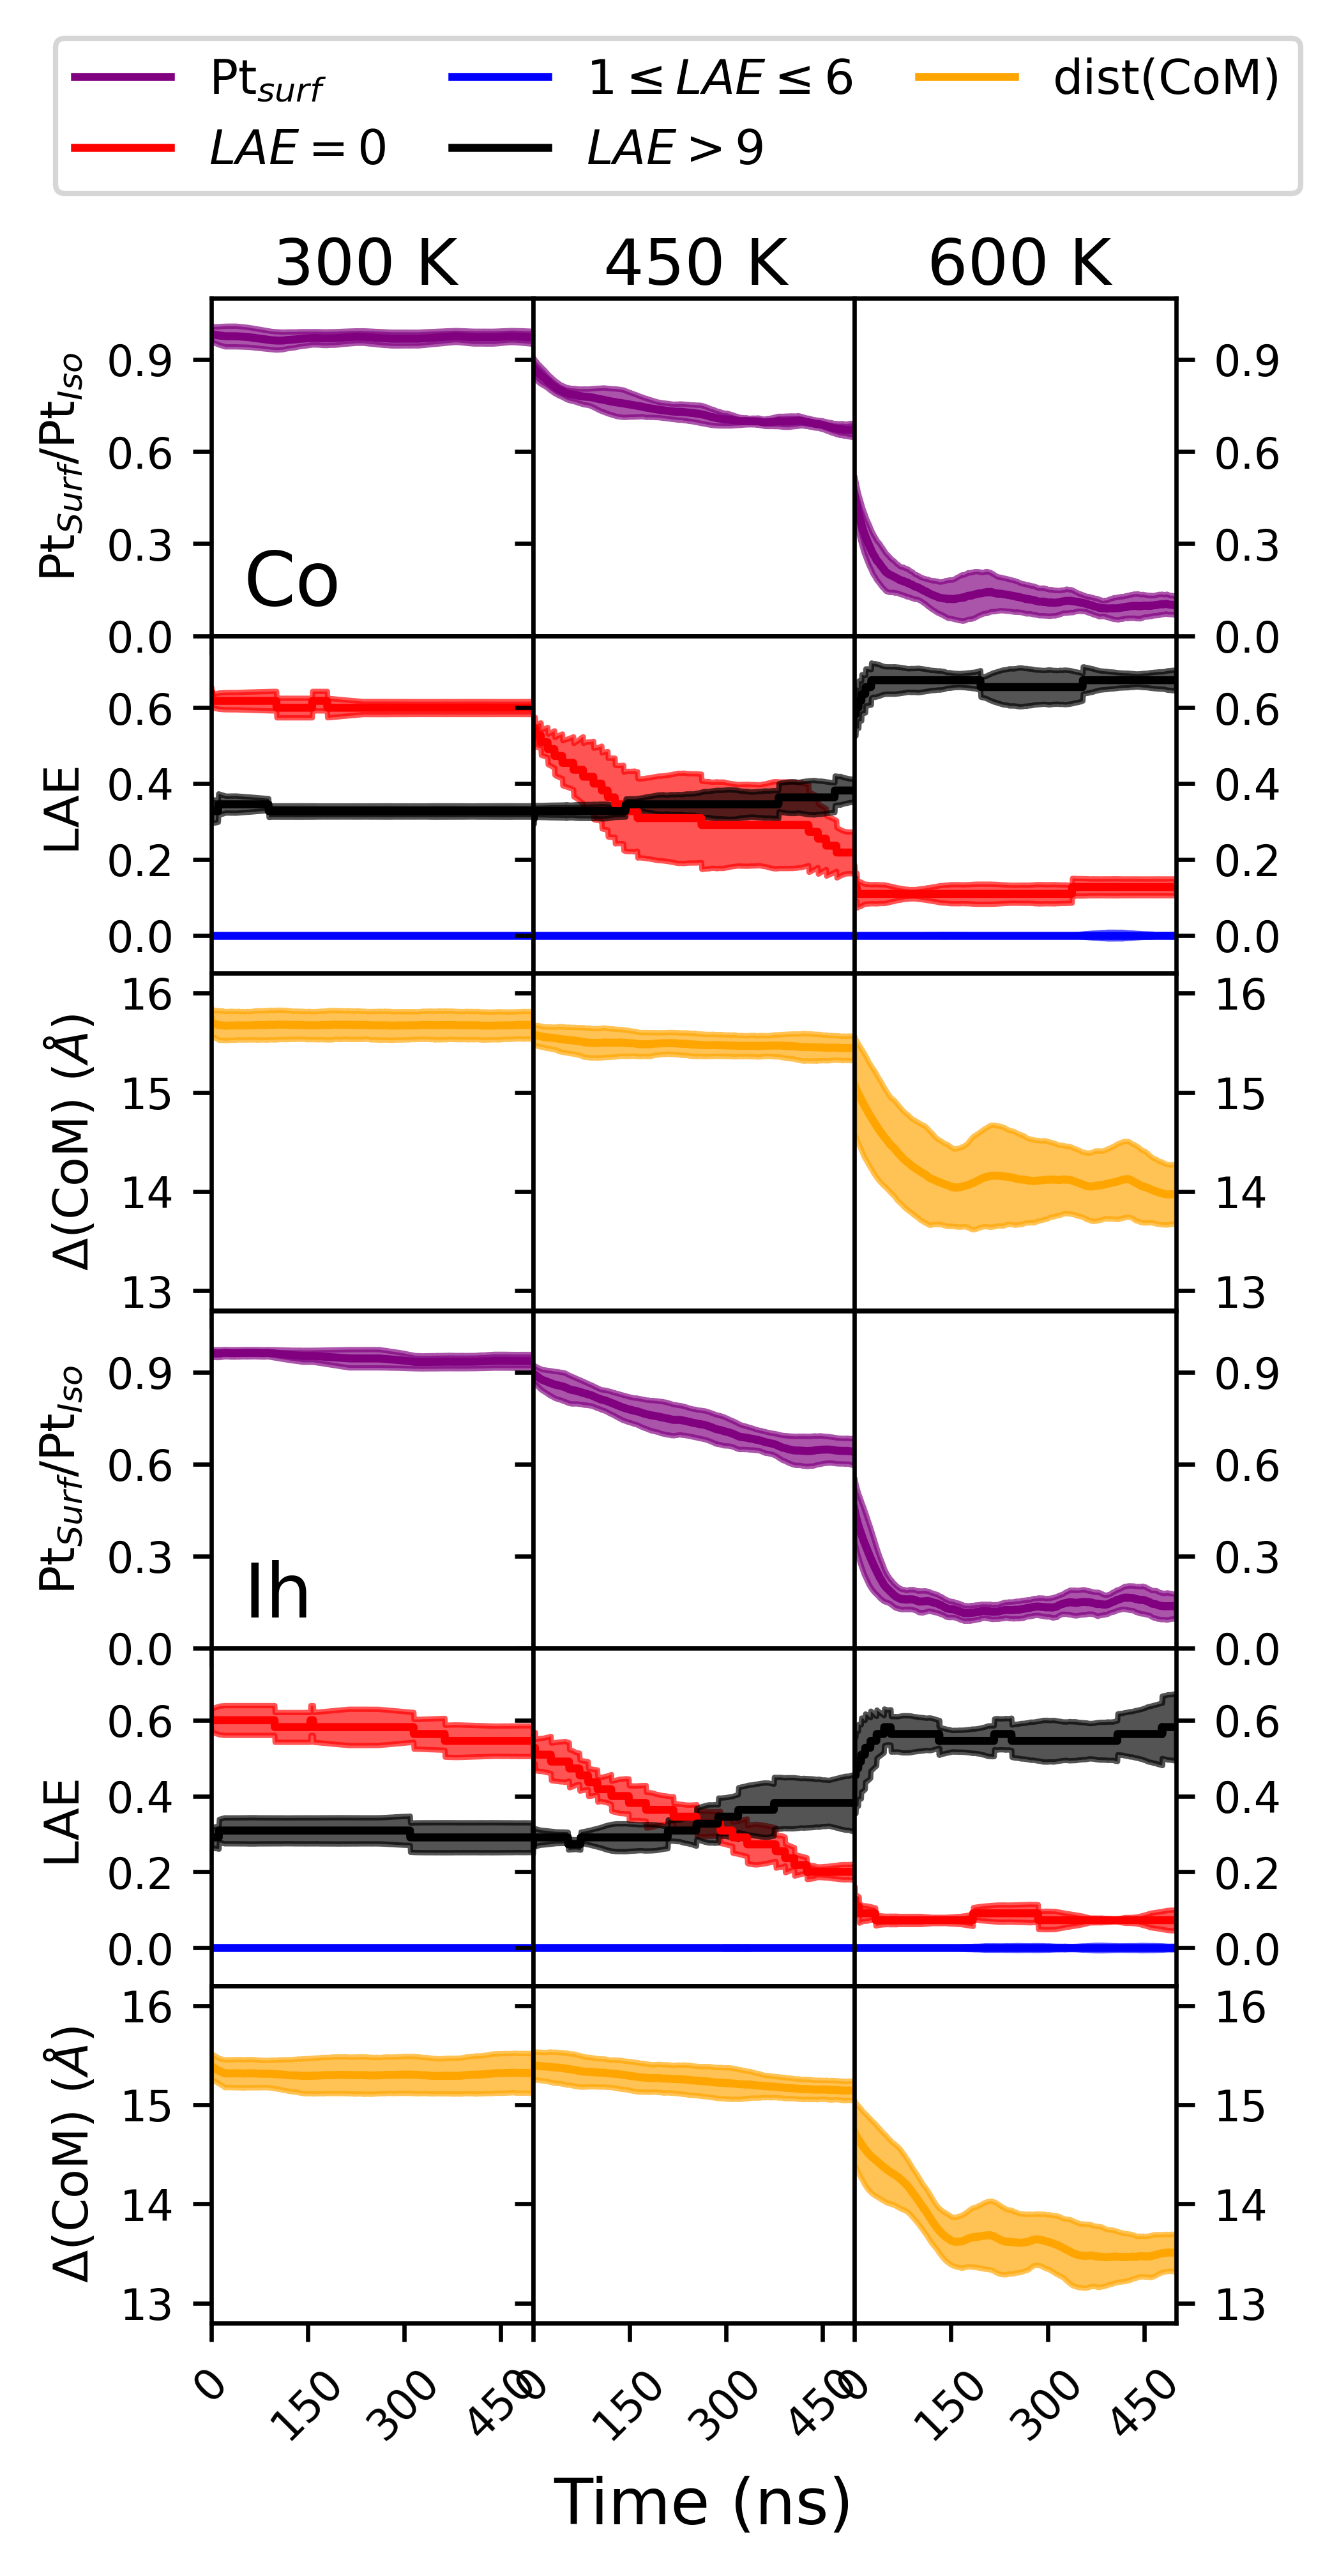
\includegraphics[width=\textwidth]{figures/MD/Coal/891.png}
         \caption{}
         \label{fig:MD_Coal_891}
     \end{subfigure}
     \hfill
     \begin{subfigure}[b]{0.31\textwidth}
         \centering
         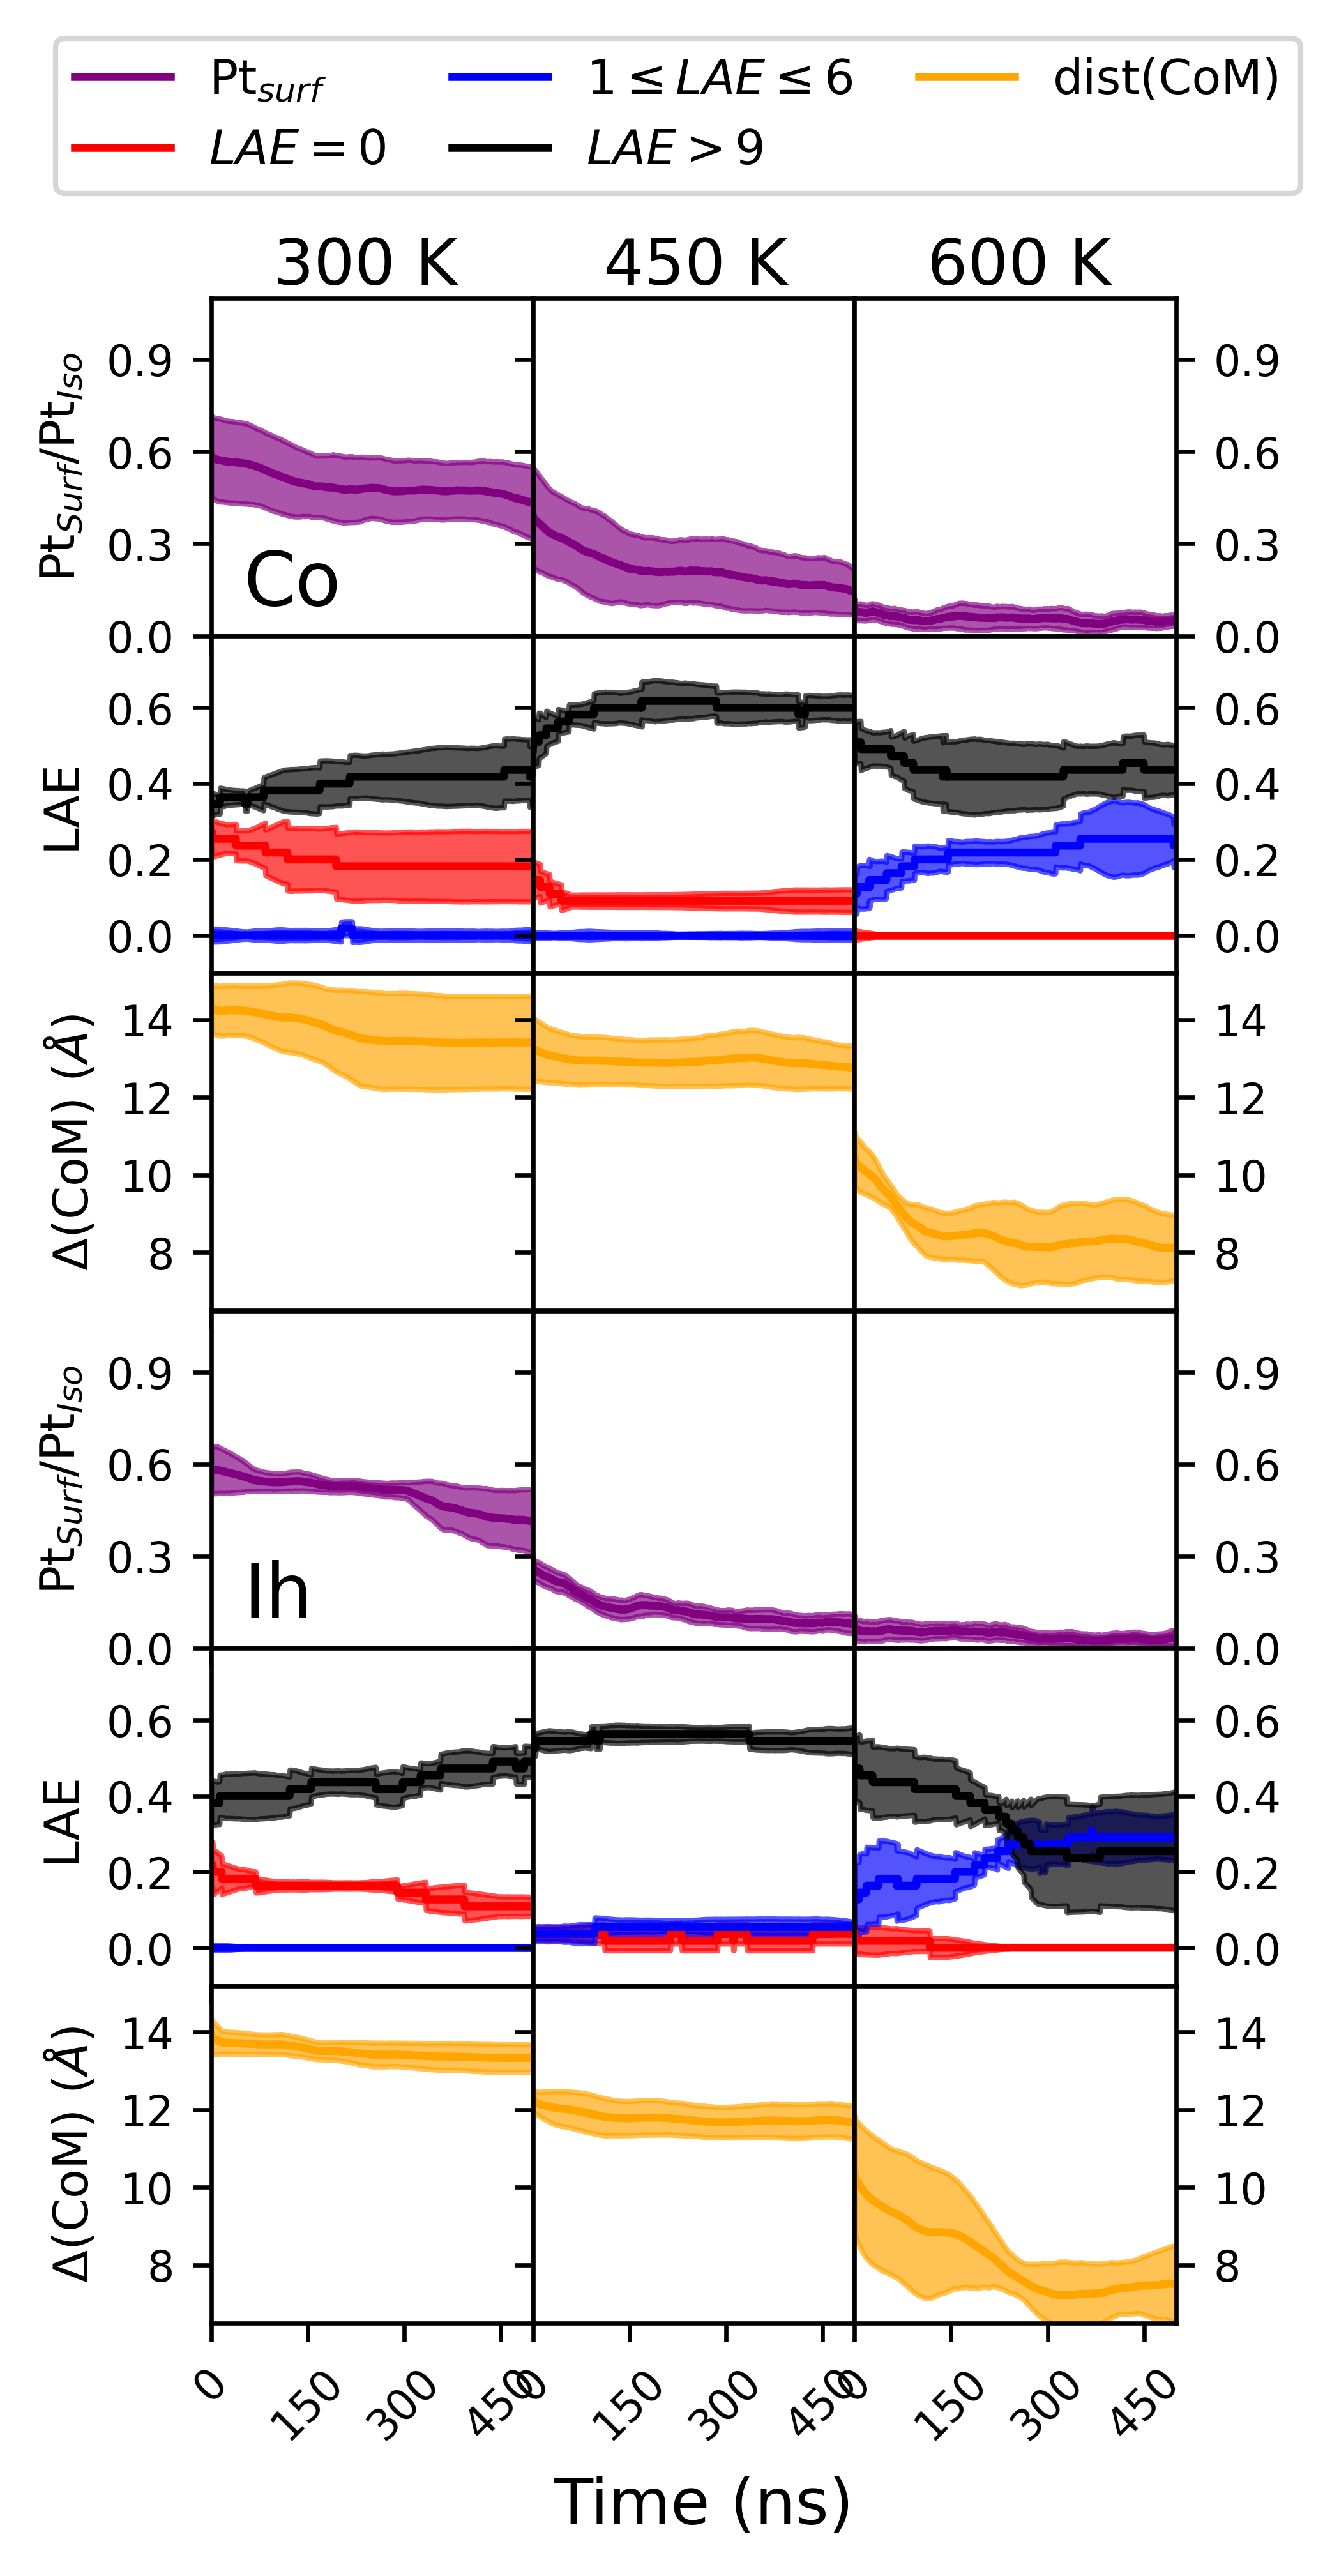
\includegraphics[width=\textwidth]{figures/MD/Coal/923.png}
         \caption{}
         \label{fig:MD_Coal_923}
     \end{subfigure}
     \hfill
     \begin{subfigure}[b]{0.31\textwidth}
         \centering
         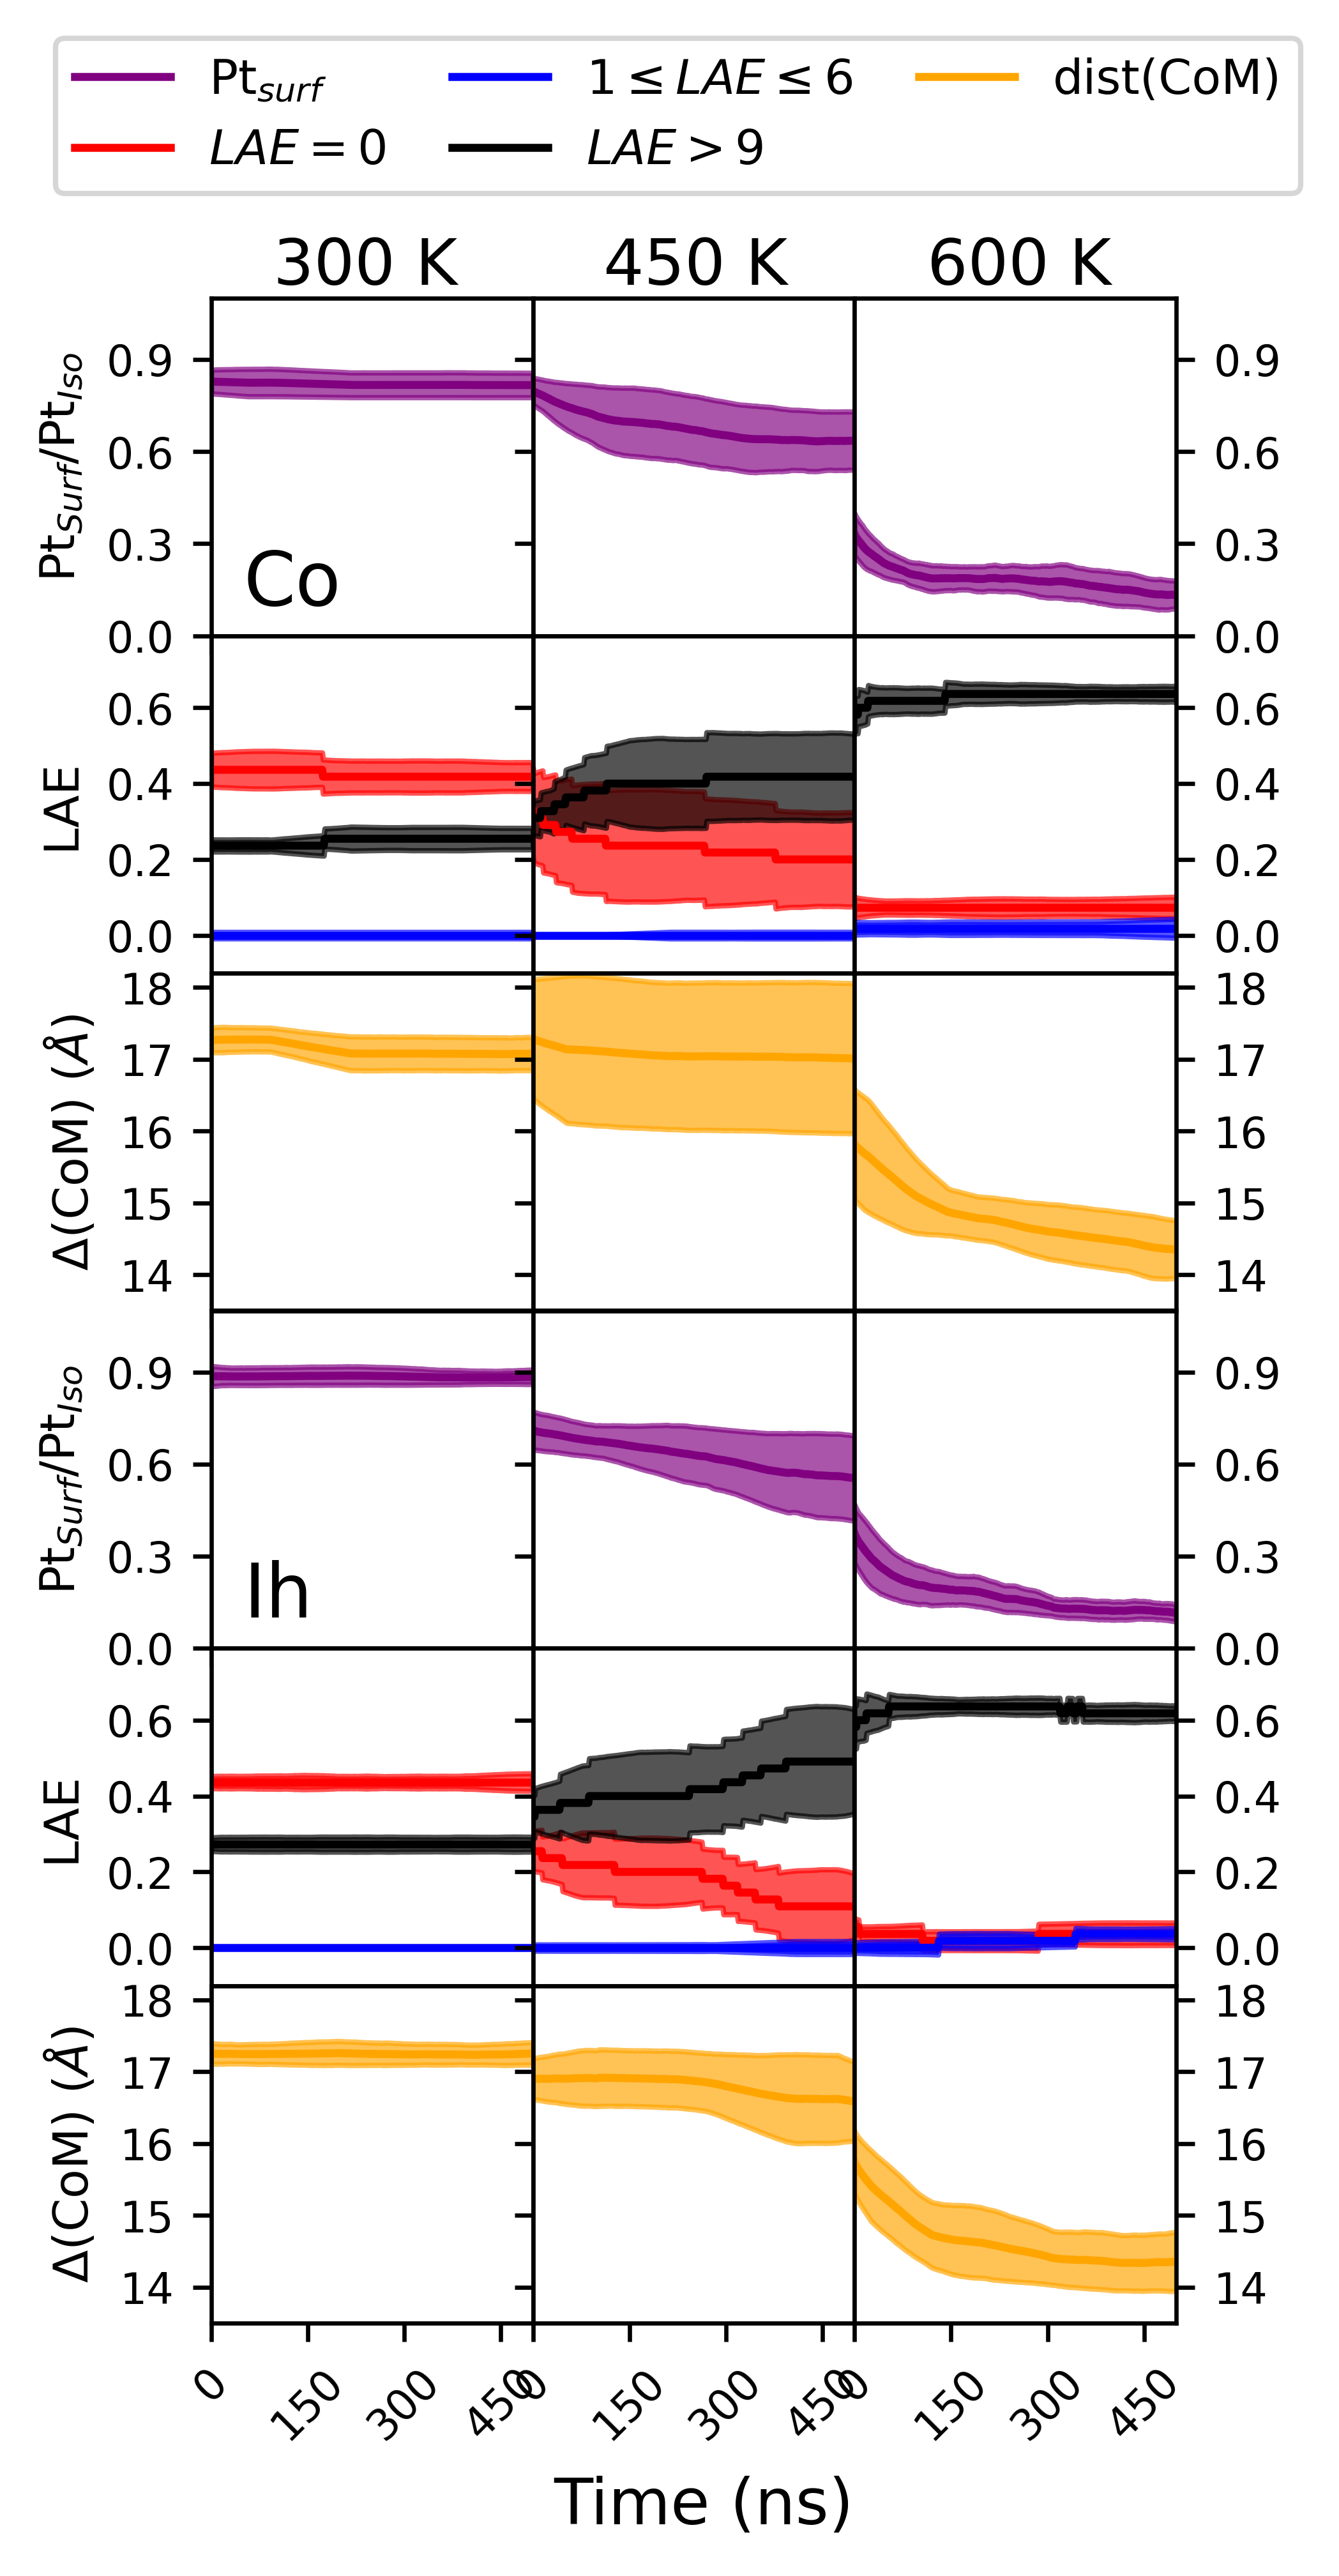
\includegraphics[width=\textwidth]{figures/MD/Coal/1103.png}
         \caption{}
         \label{fig:MD_Coal_1103}
     \end{subfigure}
    \caption{Ensemble average of time dependent descriptors of the evolution of varying AuPt NA morphologies. \textbf{a.} Au$_{891}^{Oh}$. \textbf{b.} Au$_{923}^{Ih}$. \textbf{c.} Au$_{1103}^{MDh}$ Upper set of panels are for the initial Pt$_{55}^{Co}$ morphology deposited randomly on the larger Au seed. Lower panels are Pt$_{55}^{Ih}$. In each sub-figure, scales horizontally are kept the same to more easily monitor the evolution of the given descriptor.}
    \label{fig:MD_Coal_Evo}
\end{figure}

We analyse the first 500 ns at 300 K, 450 K, and 600 K for three Au initial cores, namely the Au-Oh$_{891}$, Au-Dh$_{1103}$, and Au-Ih$_{923}$; and Pt$_{55}$. Our results are shown in the columns of Figure \ref{fig:MD_Coal_Evo}. Clearly at 300 K a few diffusion processes are activated and they are mainly mechanisms occurring at the surface. Pt decorating Au remains roughly at surface and there is little mixing. This is evidenced by all panels demonstrating a minimum of 35\% of the incumbent Pt remaining as surface-like. Only on Ih$_{923}$ there is evidence of Au beginning to cover Pt, as highlighted by the decreasing ratio of Pt atoms at the surface with respect its initial value, but still above 35\% of Pt is still at the surface before considering the relatively large uncertainties between the iterations. The Au-adatom mobility on Au-Ih suggests that adatom formation and climbing on Pt-decoration are considerably easier on that morphology. A rational behind it is that the inter-shell distance in an Ih are elongated of about the 5\% along the radial direction. 
The first large-scale rearrangements on the 0.5$\mu$s scale, occur at 450 K. The three cores behave similarly. In all cases, Pt atoms increase their average coordination and a greater occurrence of Pt has at least an Au as nearest neighbour but still a few Pt are  surrounded by Pt only.  In the case of Oh and Dh still the 45\% of Pt is at surface, although slowly decreasing, while the same percentage is about 10\% on Ih-core. 
%
We should note that surface diffusion is slow and only few Au adatoms detach and are free to hop and exchange. At 450 K, Au-climbing is activated and we observe a full or almost full encapsulation of the decorating Pt nanoparticle. In the case of Oh and Dh, the slow increase of the average coordination suggest that the encapsulation is done by Au-climbing \& diffusing and not by a concerted drop of the Pt inside the Au-core.

In all reported cases at 600 K and on a timescale shorter than 50 ns, the decorating Pt-nanoparticle becomes encapsulated as evident from the sharp increase of the average Pt coordination, the sudden drop of the relative abundance of Pt atoms without Au as nearest neighbour (LAE${Pt}_{m=0}$), and the decrease of Pt atoms that are identified as surface atoms. The latter has a behaviour that clearly differentiates the Au-core. While in Au-Ih, already after the initial stage few, if no, Pt atoms are at the surface, the lack of Pt surface-atoms on Au-Oh and Au-Dh is completed after 100~ns. 
The non-zero value of LAE${Pt}_{m=0}$ for Au-core displaying a Oh and MDh, while it is zero for Au-Ih, suggests the formation of a quasi-Janus nanoalloy, with a few Pt atoms forming only homo-pairs and hence indicates the formation of a quasi-Janus ordering.

Furthrmore at 600 K, there is a concerted motion of the Pt nanoparticle up to about 200 ns as revealed by the linear decrease of the distance between the COM of Pt and the one of the whole nanoparticle. This should support that the Pt-nanoparticle makes a concerted motion inside the Au-core. The formation of Au adatoms and vacancies favourite the Pt anchoring. Then Au adatoms climb and diffuse onto Pt. Au-adatoms climb from opposite site of the Pt-nanoparticle with a net effect of encapsulating it.
 %
 The formation of a partial onion-shell in Au-Ih is labelled by the linear increment of $LAE^{Pt}_{m\geq10}$ already in 100 ns as highlighted by the almost first order transition in the Pt average coordination and on the increasing of the ratio of Pt atoms with a more than 10 Au-atoms in the local environment. Furthermore, the absolute value of $\Delta_{COM}$ as low as 8 \AA \ reveals that Pt moves closer to the CoM of the system, further suggesting encapsulation when deposited onto an Ih.

%
\subsection{Pt-loading effect}
We study the coalescence of Pt$_{M}^{Ih}$ onto various Au$_{N}^{Ih}$ ``magic'' Ih-seeds over a period of 100 ns at 600K following the collision, with the condition $M\leq N$. Our results are summarised in Figure \ref{fig:Ptload_Data}, where we record the $\Delta (RoG)^{Pt}$, the average coordination of Pt atoms, their local atomic environments (LAE) and the relative distance of the com of the Pt atoms from the com of the whole system.

Despite the previous work revealing Ih as a seed Au to perform poorly with respect to ensuring Pt stability, we motivate our choice in studying further the Ih morphology with the work of T. Rossi \textit{et a.l} \cite{TRossi2020} which demonstrated that the Ih is indeed the most performant Au structure for generating hot carriers. Nonetheless, it remains an obvious extension to this project to consider the loading ratios on Au seeds of varied morphology to determine if the trade-off in hot carrier generation may be mitigated by having a more stable Au seed morphology. However, this too must be balanced against the consideration that the Ih is the most spherical regular polyhedron, and therefore at larger sizes is likely to be a more commonly appearing morphology under experimental conditions.

While encapsulation is likely to be observed, as revealed by the near-zero occurrence of Pt-atoms at the surface, for loading higher than 30\% the chemical ordering depends strongly on the size of the Au seed. We note that bigger the Au seed is - the dissolution, hence the formation of a POS chemical ordering, becomes increasingly retarded. By considering Pt-atoms without Au neighbours in their LAE, black markers in the lower panel, we observe a non-trivial proportion of such LAEs at loading ratios as low as 10\% on Au$_{923}$ and Au$_{1415}$ in Figure\ref{fig:Ptload_Data}, respectively). Conversely, higher loading ratios are required to observe similar behaviour for smaller Au seeds, with 50\% on Au$_{147}$ and greater than 30\% for Au$_{309}$. Motivating the assertion that there is indeed a size dependence with respect to the types of LAEs which may be formed. There appears to be a strong correlation between the $\Delta(RoG)^{Pt}$ and both the Au-seed size, and Pt-loading ratio with the latter tending to maintain the initial Pt distribution for lower loading ratios. For smaller Au seeds, there is a greater propensity for Pt atoms to be more widely distributed with respect their specie-specific CoM. As a paradigmatic example, we comment on the Pt$_{55}$ decorating Au$_{309}$ (Au about 2nm and Pt loading at 15\%). A Pt$_{55}$ is fully encapsulated inside a Au-Ih$_{147}$ and we observe even a structural reordering towards a partial onion-shell, with Pt atoms occupying subsurface positions and the overall structure is a defected and spherical Ih.

\begin{figure}
    \centering
    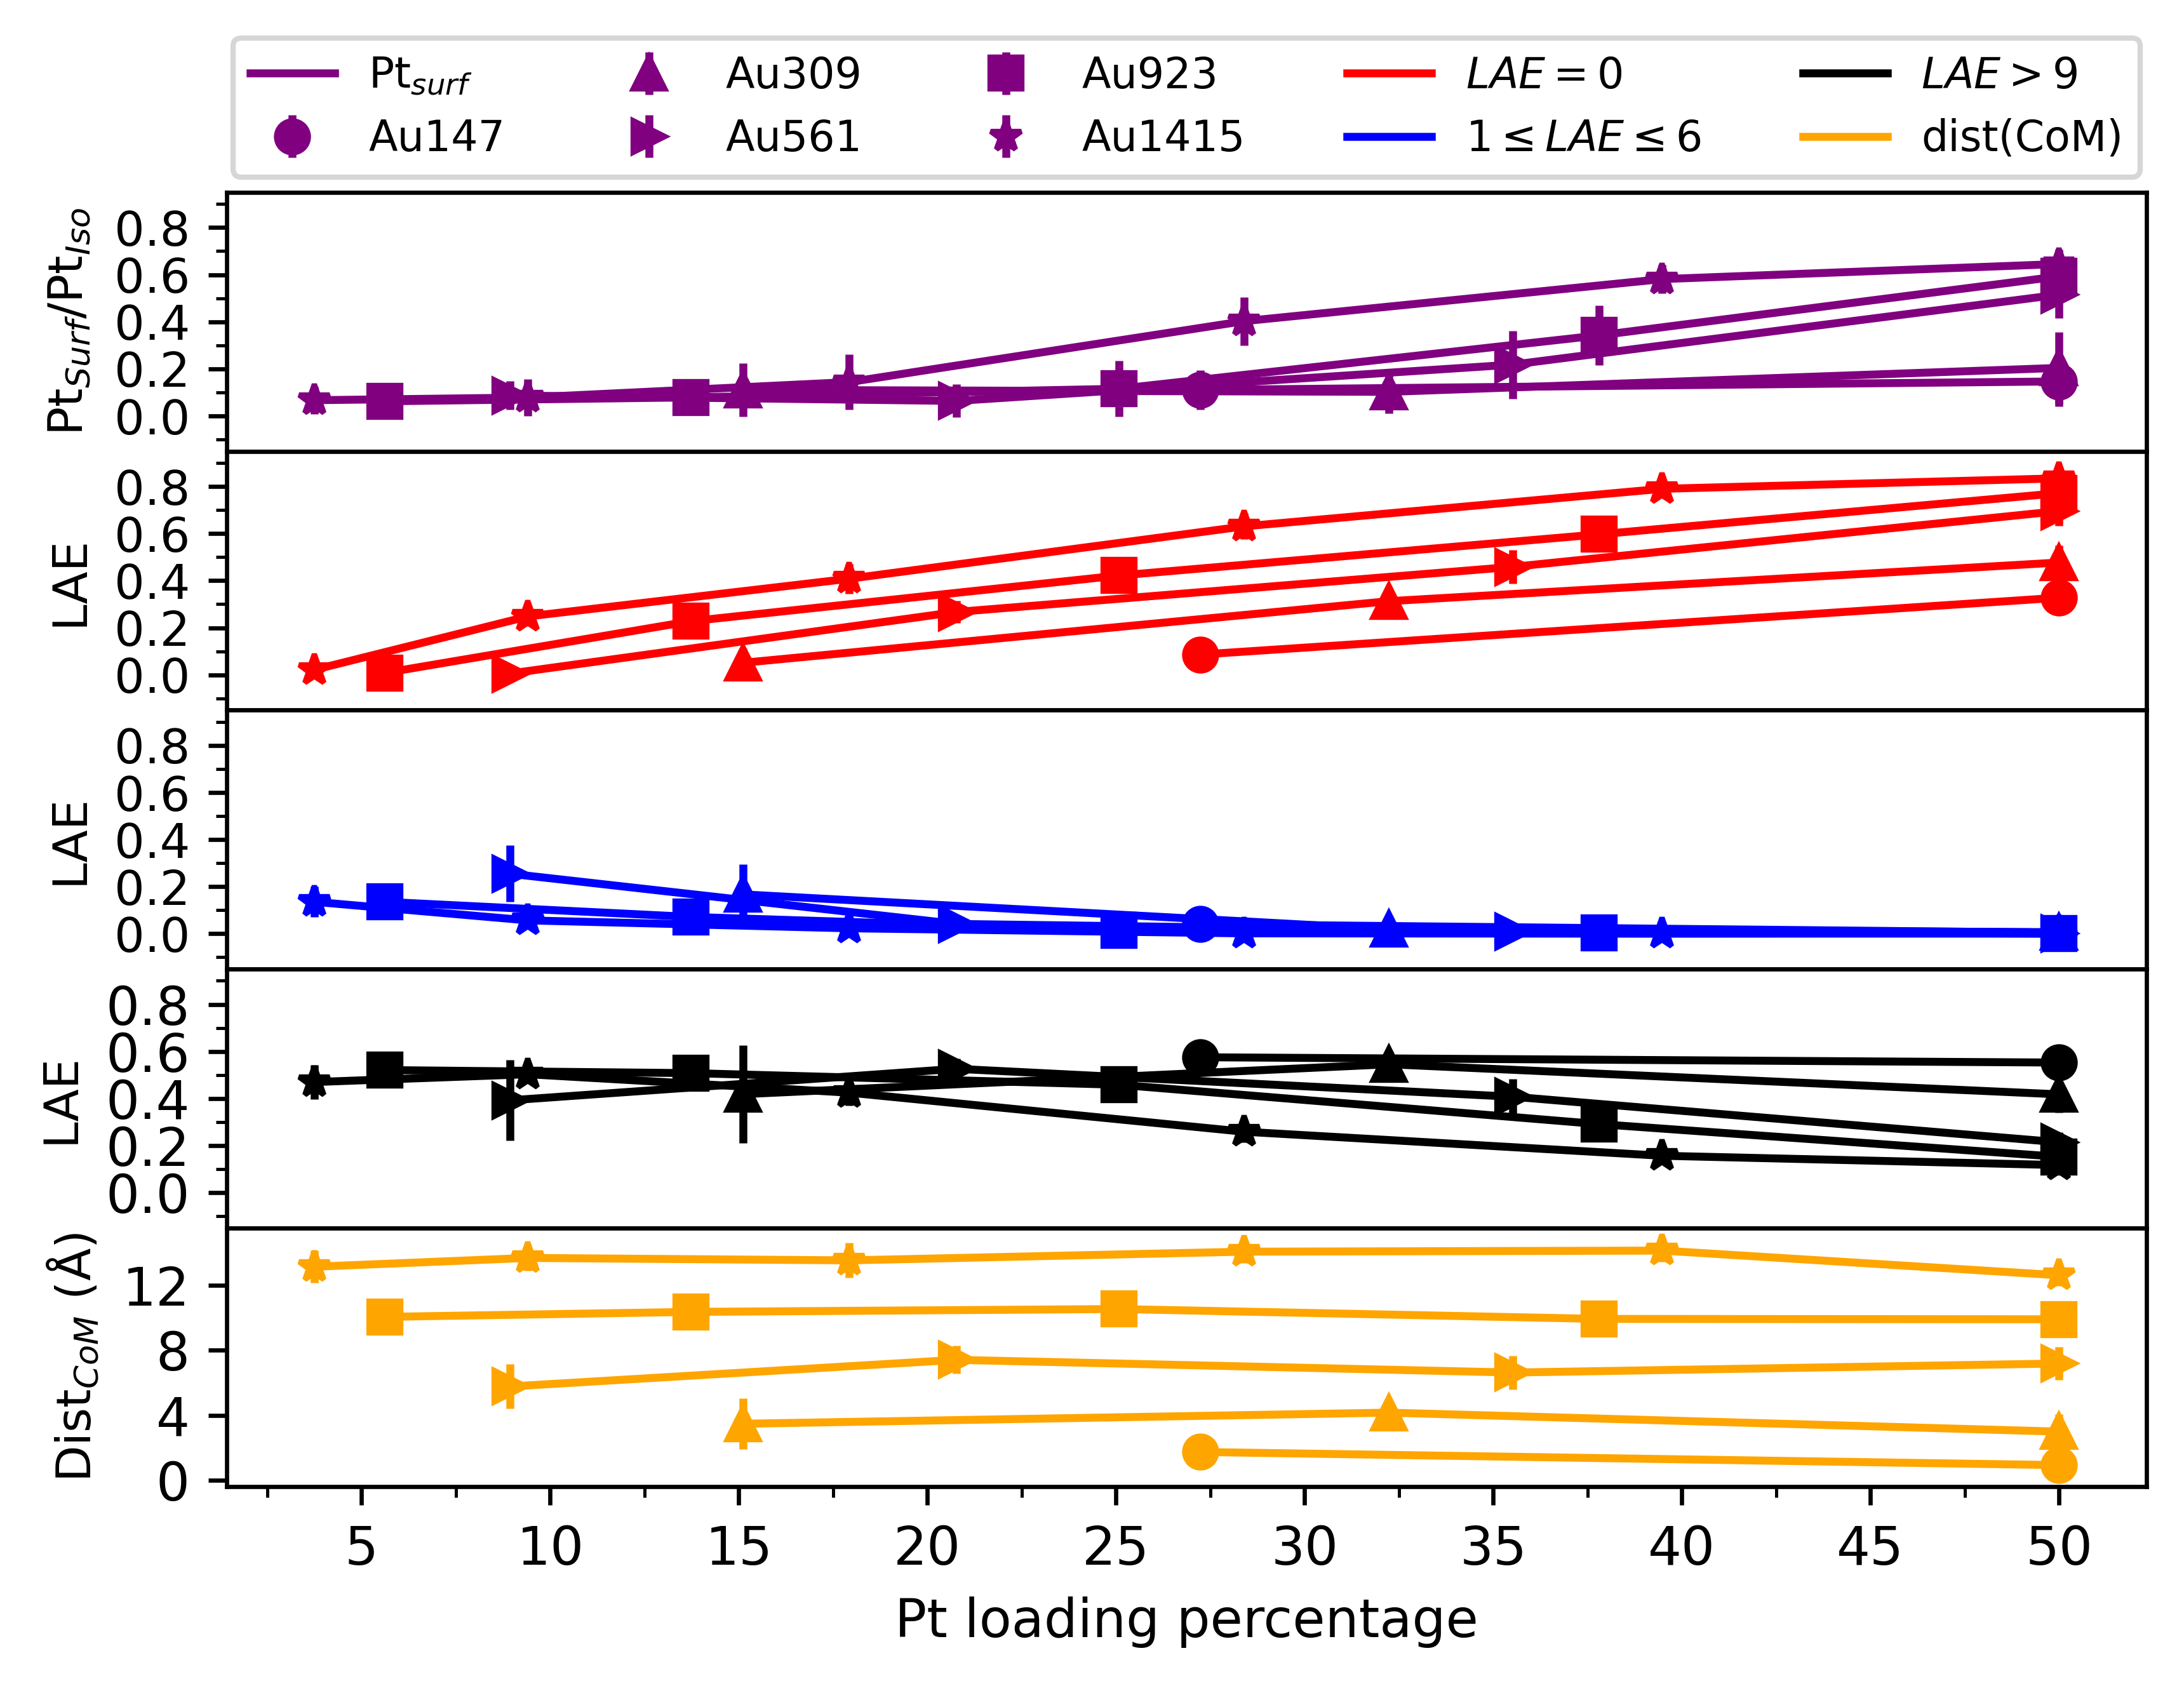
\includegraphics[width=\linewidth]{figures/MD/Coal/IhData.png}
    \caption{Variation of local and structural quantities as a function of the relative Pt loading \% discriminated by the initial Au seed. Lines on the figure follow the increased loading of a given Au seed - as denoted by each specific marker. These curves are simply an aid to the eye to track how each seed responds to increased Pt loading. Each data point is an average over the final 5 ns of the 100 ns NVT dynamics at 600 K for the specified alloy.}
    \label{fig:Ptload_Data}
\end{figure}

By considering both the top and bottom panels of Figure \ref{fig:Ptload_Data}, we may observe that all loading ratios permit the creation a partial-onion-shell like structure, this is evident in the increase in the large values for LAE$\geq$9 subject to the same arguments we previously offered. However, this shell is appearing to be several atoms thick, as indicated by the presence of a non-zero LAE=0 signature at sufficiently high loading ratios independent of size. Nonetheless, at low loading ratios, this value is near-zero for all Au seed sizes considered which suggests that small Pt decorations are unable to maintain their cohesivity at this temperatures and instead become incorporated into the larger Au structure.This is not to say that the Pt becomes completely dispersed within the Au, rather that it is becoming elongated and stretched, indicated by the $1\leq$LAE$\leq$6 signature being non-zero at these loading ratios. 

However, this signature become negligible in contribution at higher loading ratios. Moreover, for loading ratios above 30\%, there is evidence of increased Pt cohesivity and surface present given by all of the indicators presented in Figure \ref{fig:Ptload_Data} and visible in Figure \ref{fig:Ptload_Struts}. There are, however, two exceptions to this generality - the cases of Au$_{147}$ and Au$_{309}$ indicated by the circle and upward triangle respectively. Here, we may follow the seed guiding lines in the figure to reveal that even when the Pt is of an equivalent size, none of it remains surface-like. It is possible that at the temperatures studied, 600 K, this is sufficiently high to completely disorder the nanoalloy and allow it to evolve towards a deeper energy minimum otherwise inaccessible to the other clusters. As discussed in Chapter \ref{c:Theory}, the melting temperature of a cluster increases with its total size. Applying the reverse argument could lead us to the conclusion that at 600 K, the temperature is sufficiently high for the Au component to enter the liquid drop phase, and likewise too the Pt component given the evident low LAE=0 signatures identified in Figure \ref{fig:Ptload_Data}. 

On the converse, it is clear that by increasing the relative abundance of the Pt deposited onto the Au cluster, so too may we increase the efficacy of the candidate cluster as a potential nanocatalyst, given that catalytic reactions are wont to happen on the surface of the Pt more so than on Au. However, this is not necessarily an optimal solution given the rarity of Pt and its relative cost. To inspire some optimism, we do however note that larger Au clusters present more stable Pt at lower loading ratios. Take for example Au$_{1415}^{Ih}$Pt$_{561}^{Ih}$  depicted by the third downward arrow from the right in Figure \ref{fig:Ptload_Data} and visible in Figure \ref{fig:Ptload_Struts}. Whilst there is indeed strong evidence of encapsulation given the indicators, it is by no means complete given the preservation of $\sim$ 40\% of its total available surface. Moreover, it is clear that this Pt decoration is maintaining much of its own integrity despite constituting a relatively small fraction of the total cluster at 28\% of the total contribution. This is evidenced in the high ratio of LAE=0 signatures and the lowest visible LAE$\geq$9 signature for that loading ratio. Once again, this may be due to the increased stability of larger clusters on the same isotherm for the reasons provided above. Therefore, given that the Au coating Pt surface mechanism is thermally activated, this problem may be mitigated by having larger nanoalloys. However, this too is not a solution without consequence. As one decreases the absolute size of the cluster, so too does one increase the surface to volume ratio. Given that an overarching consideration is to have effective catalysts at minimal size and cost, it is undesirable to have to increase the relative abundance of Pt so as to ensure that more is able to perform its desired action.

This problem too is confounded by the fact there are two competing size scales present between the two clusters. We ideally wish to maximise the size of the Au cluster so that it may absorb more light, and therefore increase the rate of hot carrier production given that the two are inexorably linked \cite{AuPlasmonRev}. On the converse, as stated previously, we wish to minimise the amount of required Pt to be efficient with rare metals, and to increase the surface to volume ratio as sub-surface Pt is essentially inert with respect to surface catalysis. Considering these two scales in tandem, one may intuitively arrive at the conclusion that by maximising the Au size for a given cluster, and minimising the relative Pt, one may develop the ideal plasmon enhanced photo-catalyst. However, as our results have shown, this may be more an idealisation than reality. As by having ultra small Pt decorations, one is subject to surface pollution by encroaching Au atoms. Indeed, these results suggest that components must necessarily be larger if one is to design an effective catalyst.

\clearpage
\subsection{Complex decoration effect}

We study the effect of a co-assembly two Pt$_{55}$ onto a Au-Ih$_{2057}$ on opposite facets. We analyse dynamics long 500 ns, at different temperatures between 300 up to 600 K at increments of 50 K, as reported in Figure \ref{fig:micki}. At each temperature, we initiate the dynamics with the same initial structure such that we are not undergoing an iterative heating process and are rather monitoring the evolution of the nanoalloy when it is subject to different temperatures to determine the level at which different transformations may be considered to be thermally activated. As before, we consider only the Ih morphology for both the Au and Pt components of the configuration for the reasons specified above. We create these nanoalloys in much the same fashion as before. Via the soft landing of Pt onto the Au seed at random locations. We have done this is in two fashions. One where there is a single Pt cluster deposited, and a second where this is done a second time so as to imitate a more complex type of configuration which may be experimentally viable as seen in \cite{Jorge2019}. We have placed the itinerant Pt clusters far from one another so that they do not interact.

In general, we do not anticipate large deviations with respect to the structural response as was discussed earlier. Nonetheless, it will be interesting to observe whether there is any appreciable deviation from a single soft landing to multiple Pt clusters as is a common experimental practice \cite{JorgeStructure}.

\begin{figure}
\centering
    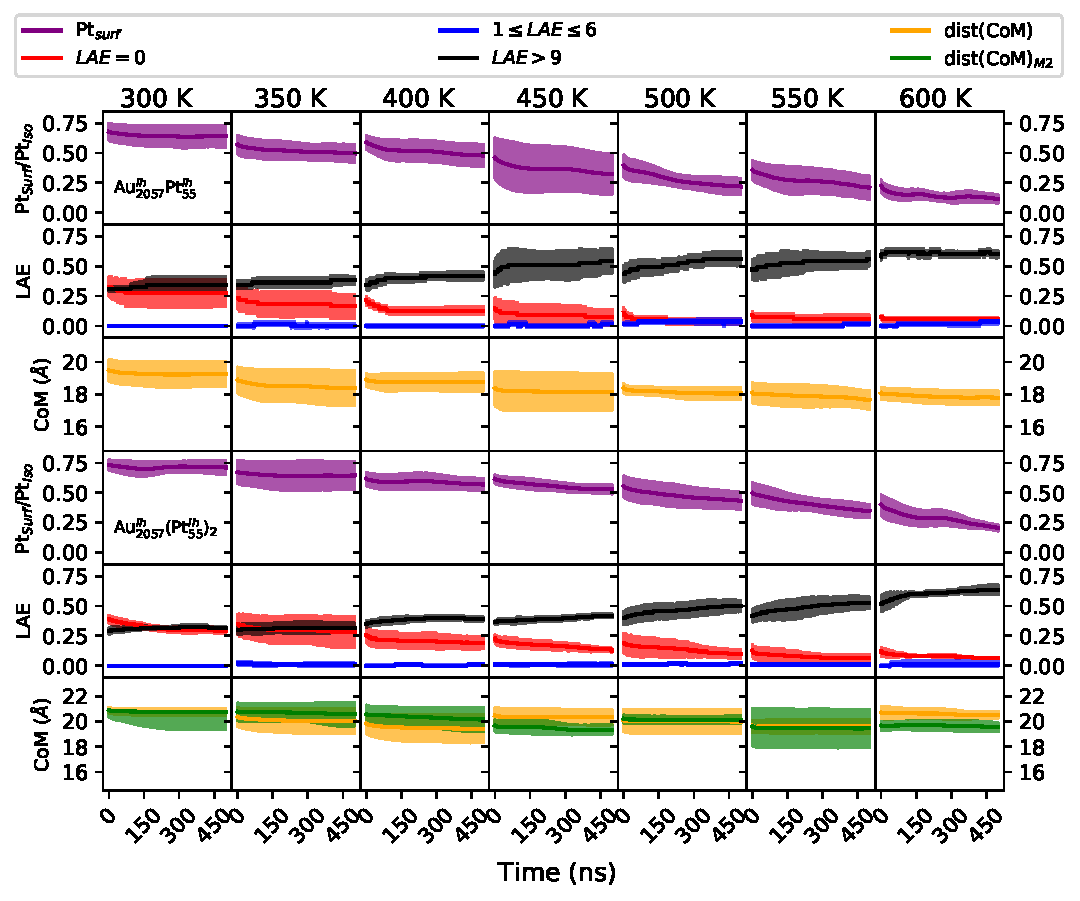
\includegraphics[width=\linewidth]{figures/MD/Coal/Micki.pdf}
    \caption{Evolution of the structural descriptors for the complex Pt loading nanoalloys featured in the bottom right of Figure \ref{fig:beginning}. Upper set of panels represent Au$_{2057}^{Ih}$Pt$_{55}^{Ih}$, and the bottom panels - Au$_{2057}^{Ih}$(Pt$_{55}^{Ih}$)$_{2}$.}
    \label{fig:micki}
\end{figure}

In a similar fashion to the dynamics demonstrated in Figure \ref{fig:MD_Coal_Evo}, it would appear that 450 K is indeed the temperature at which the restructuring of the composite alloy is truly activated. We motivate this by observing that this is the temperature where the gradient of the purple curves, representing the surface contribution of the Pt to the nanoalloy, begins to change in an appreciable fashion. Whereas at lower temperatures there is evidence of Pt stability, albeit with a gradually reduced Pt surface contribution. Nevertheless, it would seem that, as indicated by Pt enjoying an LAE$\geq$9 being lower than 50\% for all temperatures below 450 K, there is still a strong sense of cohesion within the Pt clusters for both the single deposition and the complex decoration. This is further corroborated by the LAE=0 indicator being of a similar scale to LAE$\geq$9. Recall that for an Ih$_{55}$, the inner core only consists of 13 atoms meaning that the maximal LAE=0 value in principle should be 0.25. Where there appear to be values above, this is purely a consequence of the uncertainties being reported which have naively been computed as $\pm$ the standard error across the realisations. Therefore, values above are unlikely to be meaningful.

In our comparison with the single Pt$_{55}$ decoration, we note that the encapsulation is slower when two Pt-nanoparticles are soft-landed. However, at temperatures above 500 K, it would appear that not only are the nanoparticles being encapsulated, but also that they begin to undergo a fragmentation process, suggested by the slight increase in the 1$\leq$LAE$\leq$6 at these higher temperatures and the sharp increase in LAE$\geq$9. However, there is also strong evidence for encapsulation in conjunction with this fragmentation as suggested by the decrease in CoM distance between Pt and the cluster. In general, this is only really on the order of $\sim$ 2 \AA \, which is approximately half of the radius of one of the considered Pt clusters. Curiously, this appears to be more profound for the case where two Pt clusters were deposited, where each Pt nanoparticle shifted towards the total cluster's centre of mass by 4 \AA, where we have depicted the second cluster with a green curve so that we may monitor their motion separately. It is possible that by disrupting the larger Au seed further with an additional Pt, it became more susceptible to greater surface reconfiguration which would result in an enhanced mobility of Au atoms to absorb the Pt clusters within. 

\subsection{Greens Dyadic Method}
\label{DFT:GDM}
For manifold reasons, scale being the principle driver, the use of \textit{ab initio} techniques for determining the optical properties of alloys and nanoalloys is not feasible. Moreover, whilst continuum models do exist and are commonly used to model these clusters, it is not always an optimum consideration as one loses a sense of precision when describing the morphology or non-trivial chemical ordering of structures. To expand, we may consider the complex configurations exhibited by the previously shown clusters following a dynamical process. Correctly and faithfully recreating such configurations with a continuum model would become prohibitively challenging and the recreation would only truly be in broad strokes - describing regions where there may be a greater present of one material over another, but missing the precision of features such as surface climbing and wetting that we have demonstrated occur within these systems. To provide a bridge between an atomistic, yet computationally tractable approaches, we have utilised the GDM introduced in Section \ref{sec:GDM}, developed with atomic precision in Section \ref{c:Sapphire}.

As discussed previously, this method enjoys the privileged position of maintaining a broadly atomistic description of the matter, albeit with important approximations such as treating each element as a dipole with refractive properties inherited from experimental data. However, it is not just the atomic description of nanoalloys which incites this method's appeal. We may in principle scale up the considered structures almost arbitrarily. Whilst computational constraints render the method cumbersome at over 3000 dipoles, we may vary the scaling of the size of each dipole element within the mesh. Essentially, this allows us to treat regions of the material effectively as "super dipoles" in a similar fashion to the super atom model. In that the aggregate of atomic properties may be consolidated into a single more manageable element. Whilst this indeed provides a tantalising window through which we may observe the solution to our scaling issue, it is not necessarily practical to do so to arbitrary size. As one will eventually reach a total system size which may be more efficiently treated within the scope of a mature finite element solver as one effectively loses the atomic precision at such scales which sets this method apart.

Nonetheless, this method is desirable for the structures explored in the previous sections of this chapter. We are still considering sizes where atomistic precision is desirable but an \textit{ab initio} method is unfeasible. However; the size regime considered, on the order of several nanometers, may still be considered to exhibit non-trivial quantum mechanical properties \cite{QuantumPlasmonCoupling}. Hence, we shall practice caution with these systems in the following calculations.

\begin{figure}
\centering
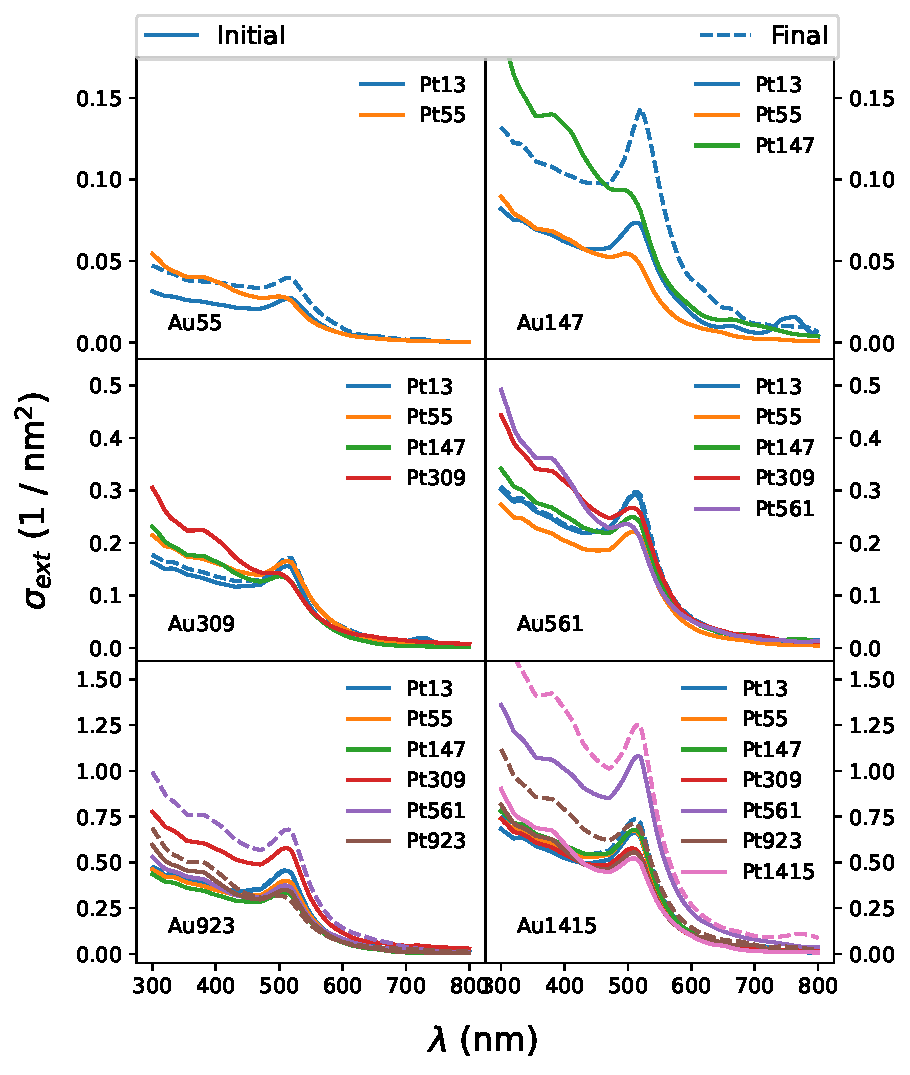
\includegraphics[width=\textwidth]{figures/MD/Coal/Specs.pdf}
\caption{Optical extinction spectra computed for the structures in \ref{fig:Ptload_Struts}.}
\label{fig:GDM_Ih}
\end{figure}

\begin{figure}
\begin{subfigure}{0.8\textwidth}
    \centering
    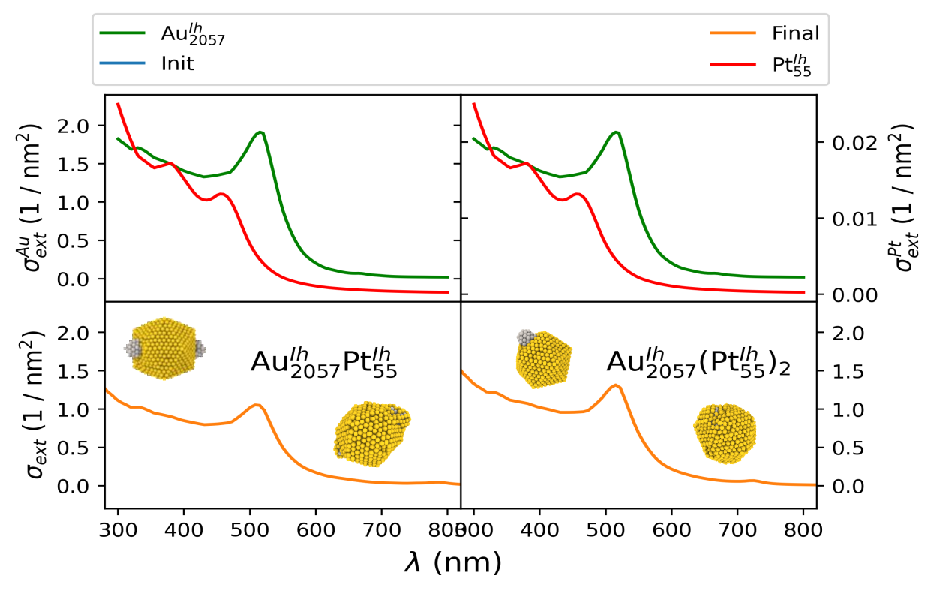
\includegraphics[width=\textwidth]{figures/MD/Coal/Micki_Specs.pdf}
    \caption{Top row of Figure \ref{fig:beginning}.}
    \label{fig:GDM_Micki}
\end{subfigure}
\begin{subfigure}{0.8\textwidth}
    \centering
    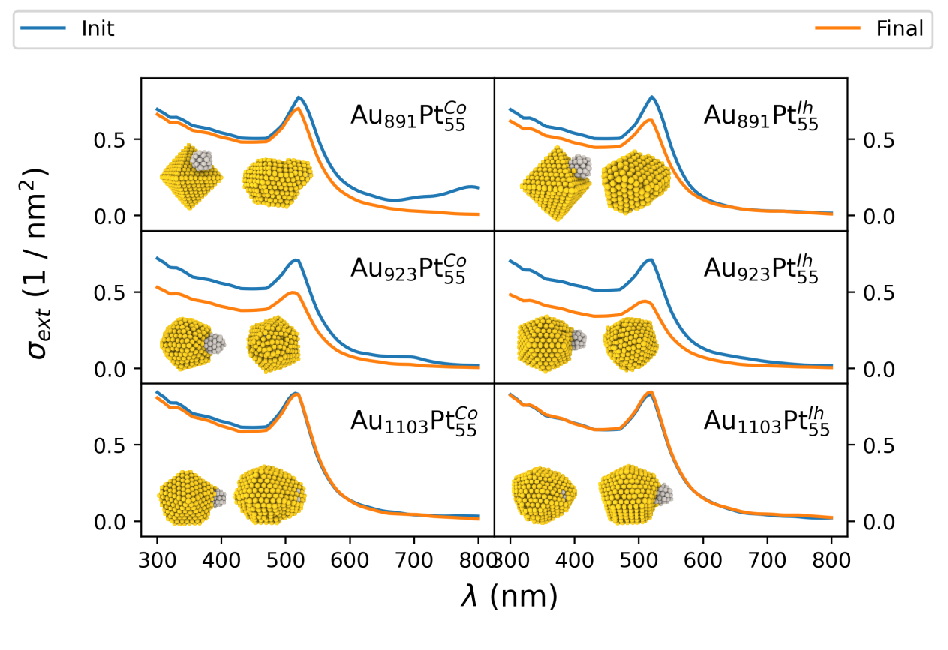
\includegraphics[width=\textwidth]{figures/MD/Coal/Seed_Spec.pdf}
    \caption{Bottom row of Figure \ref{fig:beginning}.}
    \label{fig:GDM_Long}
\end{subfigure}
    \caption{Initial and final optical extinction spectra computed for the structures identified in their respective captions before and after undergoing NVT dynamics at $600$ K.}
    \label{fig:GDM_Dyns}
\end{figure}


To compute these spectra in Figure \ref{fig:GDM_Ih} and Figure  \ref{fig:GDM_Dyns}, we have illuminated each structure along each principal Cartesian axis with plane waves $\lambda \in [300 \text{ nm}, 800\text{ nm}]$ and plotted the averaged response for each wavelength. This has been done to determine the effectiveness of our method of computing extinction spectra when compared with experimental techniques of similar structures \cite{JorgeStructure} where we identify two primary sources of dissimilarity between our system and that of the experimentalists:

\begin{itemize}
    \item Difference in size of the constituent NAs. We have Au seeds varying between $3$ - $5$ nm compared to the experimental seed which is approximately $10$ nm in diameter. A doubling in diameter approximately corresponds to an order of magnitude more material which may be influential. Moreover, their Pt decorations saw variation in shell thickness of $0.5$ to $1.5$ nm which correspond to shells many tens of atoms thick, whereas we have considered shells of up to only $3$ atoms in thickness. Alternatively, the solid Pt objects deposited atop the Au seed vary from $2$ to $3$ nm in radius. Again, an order of magnitude more material than we have considered. For reference, see \cite{JorgeStructure}.

    \item We have considered the environment for our NAs to be a vacuum - consistent with the dynamical simulations we have performed. Conversely, in the work in \cite{JorgeStructure}, the NAs were solvated in a methyl blue marker solvent to monitor the catalytic activity of the NAs.
\end{itemize}

Given these simplifications of our model, we maintain that this is not unreasonable given that we have selected refractive data to inform our model from Johnson and Christie's seminal work \cite{PhysRevB.6.4370}. Meaning that our structures inherit the optical properties of the structures investigated in the aforementioned work. Indeed, as shall demonstrate in this section, the size of the object considered in our model has minimal influence on the computed spectral properties. Instead, as we remarked in Sec. \ref{sec:GDM}, the real issue with this model manifests as we shrink the size of the NA as quantum mechanical properties begin to appear at the precise size range we consider in this project. Therefore, we must practice caution when considering NAs at or below the size range of $5$ nm in diameter, as discussed in Sec. \ref{sec:plasmons}. Furthermore, as we demonstrated in Sec. \ref{DFT:GDM}, there is little calculable influence on the optical extinction spectra for a given NA when the environment is altered. As described before, this is because the model assumes that the environment is, for all intents and purposes, homogeneous in its refractive index, and so there may be some modulation in the appearance of the primary extinction peak but this will be superficial. Rather we have elected to consider the refractive index $n = 1$, the vacuum, for the reason described above - our dynamics were run in vacuum and our extinction spectra should be consistent with this.


As we observe in Figure \ref{fig:GDM_Dyns} there are indeed observable variations in the optical extinction spectrum with respect to the style of Pt introduction, and indeed the relative loading - most evident in Figure \ref{fig:GDM_Ih} where we observe that larger quantities of Pt increase the extinction at shorter wavelengths. This may be easily intuited given that Pt is more optically active at these shorter wavelengths, albeit with significantly smaller values in extinction cross section relative to Au. Nonetheless, this is observable in our model and, more importantly, is also observable in the corresponding extinction spectra reported in \cite{JorgeStructure}. Furthermore, in the referenced work, there were reported computationally derived spectra, evaluated with a finite difference model wherein the material properties were fed into the corresponding regions. Consequently, it should not be too surprising to see similarities between these spectra and those reported here - as the models are similar in effect albeit not in technique.

Furthermore, another property is evident in the spectra reported in Figure \ref{fig:GDM_Dyns}, that there do appear to be some distinctions between the spectra of the initial near-perfect objects and the final disordered NAs. By considering  where these differences are visible in conjunction with their respective NA configurations, one may infer that the primary mechanism for altering the extinction spectrum is the relocation of material on aggregate. In particular, these deviations are more profound when the Pt decoration is large relative to the Au and the encapsulation of Pt by the Au is complete or near-complete. See for example the upper four panels of Figure \ref{fig:GDM_Long} where there is a significant redistribution of Au to cover the Pt. It is likely that the nature of the model itself is responsible for these profound variations in the extinction spectra in that we have elected to use refractive index properties for the entirety of the sample considered in the reference investigation \cite{PhysRevB.6.4370}. Consequently, the model may not be able to full distinguish between the thickness of the matter, whereas its location and available surface is more important. Therefore, by drawing Au from the core of the seed to cover the Pt, and thus exposing itself more to the plane waves incident upon it.

\subsection{Discussion}

In general, we expect the AuPt nanoalloy to adopt the morphology of the Au-core with no significant structural rearrangements of the whole system occur. On the other hand, within a  timescale of 0.5 $\mu$s or shorter, we observe two general tendencies in the chemical re-ordering, namely the formation of a quasi-Janus Pt-core@Au-shell, and a partial-onion-shell (POS), depending on the Au-core morphology, and the Pt-loading. For Pt loading less than or equal to 50\%, as considered here, the expected chemical ordering, namely the onion-shell, as from global optimization studies, \cite{Deng2010} is not always formed. We observe a kinetic trapping in  quasi-Janus motif, named after the growth of AgCo\cite{Parsina2010}, which refers to a chemical distribution where the centre of mass of the Pt and Au clusters are displaced and the Pt is covered by a thin Au-layer. 
%
First, we note the formation of a (meta)-stable quasi-Janus where the Pt-NP is encapsulated and covered by a Au-skin just one-atom thick. The encapsulation is due to Au adatoms formed after the coalescence and climbing over the Pt-NP. The AuPt nanoalloy seems to remain trapped in such ordering, especially in non-icosahedral Au-cores and at low temperatures. 
However, decorating gold icosahedra (Ih), after the encapsulation, Pt atoms dissolve in and around the sub-surface shell, leading to a partial onion-shell  formation. Pt-atoms start to detach from their original structure and dissolve/diffuse in the subsurface layer of the whole nanoparticle. Such diffusion process is much faster in Ih Au-core than in any other morphology, e.g. FCC as octahedra (Oh) and decahedra (Dh), facilitate by the shell-structure characteristic of the Ih and by the elongated intra-layer distances.

%
By molecular dynamics simulations, we predict the instability of Pt-decorated (about 1 nm) Au nanoparticles (between 1.5 to 4.6 nm) in vacuum. We show which styles of chemical ordering are most likely to occur as a function of the Au morphology, temperature, and Pt-loading. Our primary focus has been on low Pt-loading, less than 50\%, to keep our structures consistent with those in the experimental literature, in absence of ligands which may significantly alter the surface energy of Au and Pt. Though our metastable quasi-Janus and partial onion-shell are the most likely chemical ordering. In both cases, a Au-skin of just one layer is formed in agreement with the general trend to have a surface layer rich of the metal with lower surface energy and larger atomic radius. We also reveal  the time scale of these chemical re-ordering, being less than 100ns at 600 K. The further diffusion and dissolution of Pt atoms inside the Au core depends on the Au morphology, with icosahedra more likely to facilitate the formation of a Pt-subshell. We investigate the atomistic  mechanism proceeding from Au adatoms which climb and diffuse onto the decorating Pt-nanoparticles and the concerted motion of Pt-diving into Au surface and sub-surface, because the formation of an Au-vacancy close to the Pt-edge. Our numerical predictions shows chemical features that can alter and even determine the lifetime of plasmonic nanocatalysts. In this respect, our predictions may guide future rational design of heterostructures made of decorating Pt-nanoparticles of Au-plasmonic cores.
